\documentclass[11pt,a4paper]{article}
\usepackage[sc]{mathpazo}\linespread{1.05}
\usepackage[margin=2.5cm]{geometry}
\usepackage{amsmath,amssymb,amsthm,mathtools}
\usepackage{booktabs,array,multirow}
\usepackage{graphicx}
\usepackage{algorithm}
\usepackage[noend]{algpseudocode}
\usepackage{listings}
\usepackage{xcolor}
\usepackage{caption}
\usepackage{tikz}
\usetikzlibrary{positioning,arrows.meta,fit,backgrounds}
\usepackage[hidelinks]{hyperref}
\usepackage{cleveref}
\usepackage[section]{placeins}
\usepackage{enumitem}
\setlist{itemsep=2pt,topsep=4pt}

\definecolor{codebg}{HTML}{F6F6F4}
\definecolor{boxbg}{HTML}{EEF4FB}
\definecolor{accent}{HTML}{2A78D6}
\definecolor{C2orange}{HTML}{EB6834}
\lstset{basicstyle=\ttfamily\footnotesize, backgroundcolor=\color{codebg}, frame=single, rulecolor=\color{black!15},
  columns=fullflexible, keepspaces=true, breaklines=true, showstringspaces=false, language=Python,
  keywordstyle=\color{black}\bfseries, commentstyle=\color{black!55}\itshape}
\captionsetup{font=small,labelfont=bf}

\newtheorem{lemma}{Lemma}
\newtheorem{proposition}{Proposition}
\theoremstyle{definition}
\newtheorem{example}{Example}
\newtheorem{remark}{Remark}

\newcommand{\Oh}{\mathcal{O}}
\newcommand{\eps}{\varepsilon}
\renewcommand{\Re}{\operatorname{Re}}
\newcommand{\ii}{\mathrm{i}}
\newcommand{\dd}{\mathrm{d}}

% a light box for key ideas
\newcommand{\keyidea}[1]{\par\smallskip\noindent\colorbox{boxbg}{\parbox{\dimexpr\linewidth-2\fboxsep}{\small #1}}\par\smallskip}

\title{Fast Evaluation of Geomagnetic Field Models\\at Scattered Points\\[6pt]
\large A step-by-step guide to the fused two-dimensional transform}
\author{Algorithm description, analysis and benchmarks\\[2pt]\small reference implementation: \texttt{fastfield.py}}
\date{10 October 2026}

\begin{document}
\maketitle

\begin{abstract}
Models of the Earth's internal magnetic field, such as the IGRF and CHAOS, are sums of spherical harmonics. Evaluating
a model of maximum degree $L$ at $M$ arbitrary points by summing all terms costs about $ML^2$ operations. For a
lithospheric model with $L=185$ and millions of satellite measurements, this takes minutes to hours. This document explains, step by step,
a method that brings the cost per point down to a few hundred to a few thousand operations, \emph{independent of $L$},
after a set-up of about one second. The method has five steps:
\begin{enumerate}[label=(\arabic*),leftmargin=2.2em]
\item separate the radial dependence into a handful of optimal radial functions;
\item rewrite the angular parts exactly as two-dimensional Fourier series;
\item ``pre-sharpen'' these series and store them on a fine grid;
\item keep only the half of the grid that is actually needed;
\item evaluate each point with a small weighted sum over nearby grid values.
\end{enumerate}
The only approximation is the finite size of that sum; its error falls by roughly a factor of ten for each extra grid point used.
Steps 3 and 5 together form a non-uniform fast Fourier transform (NUFFT) whose FFT is done in advance, with a window-sum loop built for this
problem. For $L=185$ and $10^6$ points, the method is $201\times$ faster than the direct sum at a relative accuracy of $10^{-6}$, $98\times$ faster
at $10^{-10}$, and $65\times$ faster at $3\times10^{-14}$, which is as accurate as the direct sum itself in double precision. A general NUFFT
library can perform the window sums too, but because it cannot exploit the structure of this problem it is about $1.4\times$ slower.
For the degree-13 IGRF alone, the direct sum remains competitive. The document assumes only undergraduate calculus,
linear algebra and some familiarity with Fourier series.
\end{abstract}

\tableofcontents

%=====================================================================
\section{Introduction}\label{sec:intro}
%=====================================================================

\subsection{The problem}
Satellites such as \O rsted, CHAMP and Swarm measure the magnetic field millions of times per year. Geophysicists
compare these measurements with \emph{field models}: formulas that predict the field at any position. The standard
models, the International Geomagnetic Reference Field (IGRF)~\cite{alken2021} and the CHAOS series~\cite{finlay2020}, are
written as sums of \emph{spherical harmonics}. To use them we must evaluate the model at every measurement position,
which may be millions of times, and inside an inversion this happens again and again.

\subsection{Why the direct sum is expensive}
A model of maximum degree $L$ has $L(L+2)$ coefficients: 195 for IGRF ($L=13$), and 34\,595 for the static
lithospheric part of CHAOS ($L=185$). Evaluating the model at one point means summing all of these terms, each
multiplied by a Legendre function and a sine or cosine. The cost per point therefore grows like $L^2$, and the total
cost for $M$ points like $ML^2$. For $L=185$ and $M=10^6$ points our optimised direct code takes about 86 seconds on
two CPU cores; $10^8$ points would take several hours.

\subsection{The idea in one paragraph}
Most of the work in the direct sum is repeated: neighbouring points need almost the same combination of
harmonics. The method in this document does that common work once. It turns the model into a set of values on a
fine regular grid. After that, evaluating a point only requires a small weighted sum of grid values near the point,
for example $11\times11$ of them, no matter how large $L$ is. The grid values are not ordinary samples of the field.
They are ``pre-sharpened'' so that this short weighted sum reproduces the model to any desired accuracy.

\subsection{What you get}
For $L=185$ and $10^6$ points (\cref{sec:results}), the speedup over the direct sum is:
\begin{itemize}
\item $201\times$ at a relative accuracy of about $6\times10^{-7}$ (about $0.04$\,nT on a 60\,000\,nT field);
\item $98\times$ at about $2\times10^{-11}$;
\item $65\times$ at $3\times10^{-14}$, the same accuracy as the direct sum computed in double precision.
\end{itemize}
The set-up takes about one second and is repeated only when the model changes.

\subsection{How to read this document}
\Cref{sec:background} reviews the field model and Fourier series. \Cref{sec:overview} gives an overview of the
method, and \cref{sec:step1,sec:step2,sec:step3,sec:step4,sec:step5} explain the five steps in turn. Each step says
\emph{what} is done, \emph{why} it works and \emph{how} it is computed. \Cref{sec:algorithm} collects everything into
two algorithms, and \cref{sec:parameters,sec:cost,sec:accuracy,sec:results} cover parameter choices, cost, accuracy and
benchmarks. The appendices contain the Legendre recursions, a description of an earlier three-dimensional version of
the method, and some background on why fast methods for scattered points always need one approximate step.

%=====================================================================
\section{Background}\label{sec:background}
%=====================================================================

\subsection{The internal field model}\label{sec:model}
We use spherical coordinates centred on the Earth: radius $r$, colatitude $\theta\in[0,\pi]$ (angle from the North
pole) and longitude $\varphi$. Outside the Earth, where there are no electric currents, the internal magnetic field
is the negative gradient of a scalar potential, $\mathbf B=-\nabla V$, with
\begin{equation}\label{eq:V}
V(r,\theta,\varphi)=a\sum_{n=1}^{L}\sum_{m=0}^{n}\Big(\frac ar\Big)^{n+1}
\big[g_n^m\cos m\varphi+h_n^m\sin m\varphi\big]\,P_n^m(\cos\theta).
\end{equation}
Here $a=6371.2$\,km is the reference radius, $g_n^m$ and $h_n^m$ are the Gauss coefficients (in nT) supplied by the
model, $n$ is the \emph{degree} and $m$ the \emph{order}. The $P_n^m$ are the Schmidt semi-normalised associated
Legendre functions. They can be computed by simple recursions (\cref{app:recursions}).

Throughout we write
\begin{equation}
u=\frac ar,\qquad \gamma_n^m=g_n^m-\ii\,h_n^m .
\end{equation}
Since $g\cos m\varphi+h\sin m\varphi=\Re(\gamma\,e^{\ii m\varphi})$, complex numbers let us handle $\cos$ and $\sin$
together. Taking the gradient of~\eqref{eq:V} gives the three spherical components of $\mathbf B$:
\begin{align}
B_r&=-\frac{\partial V}{\partial r}=\Re\sum_{n,m}u^{n+2}\,\gamma_n^m\,(n+1)\,P_n^m(\cos\theta)\,e^{\ii m\varphi},\label{eq:Br}\\
B_\theta&=-\frac1r\frac{\partial V}{\partial\theta}=\Re\sum_{n,m}u^{n+2}\,\gamma_n^m\,\Big(-\frac{\dd P_n^m}{\dd\theta}\Big)\,e^{\ii m\varphi},\label{eq:Bt}\\
B_\varphi&=-\frac{1}{r\sin\theta}\frac{\partial V}{\partial\varphi}=\Re\sum_{n,m}u^{n+2}\,\gamma_n^m\,\Big(-\ii m\,\frac{P_n^m(\cos\theta)}{\sin\theta}\Big)\,e^{\ii m\varphi}.\label{eq:Bp}
\end{align}
(The North, East and downward components are $B_N=-B_\theta$, $B_E=B_\varphi$ and $B_C=-B_r$.) All three have the same
shape, which we will use repeatedly:
\begin{equation}\label{eq:shape}
\boxed{\;B_c=\Re\sum_{n=1}^{L}\sum_{m=0}^{n}\underbrace{u^{n+2}}_{\text{radial}}\;\gamma_n^m\;\underbrace{\Theta_c^{nm}(\theta)}_{\text{colatitude}}\;\underbrace{e^{\ii m\varphi}}_{\text{longitude}},\qquad c\in\{r,\theta,\varphi\},\;}
\end{equation}
with $\Theta_r^{nm}=(n+1)P_n^m$, $\Theta_\theta^{nm}=-\dd P_n^m/\dd\theta$ and $\Theta_\varphi^{nm}=-\ii m\,P_n^m/\sin\theta$.

\begin{remark}[The direct sum]
Evaluating~\eqref{eq:shape} at one point means computing all $P_n^m$, their derivatives, $\cos m\varphi$, $\sin m\varphi$ and $u^n$ by
recursion, then summing about $L^2/2$ terms. This is what our ``direct'' reference code does, as efficiently as possible:
compiled, multithreaded, with pole-safe recursions. It agrees with the official IGRF software to $10^{-10}$\,nT.
\end{remark}

\subsection{Fourier series, trigonometric polynomials and the FFT}\label{sec:fourier}
A \emph{trigonometric polynomial} of degree $N$ is a function
\begin{equation}\label{eq:trig}
f(x)=\sum_{k=-N}^{N}c_k\,e^{\ii kx},
\end{equation}
which is $2\pi$-periodic. Two facts about them are used throughout.
\begin{lemma}[Exact sampling]\label{lem:sampling}
If $f$ has degree $N$ and $n\ge2N+1$, the coefficients are recovered exactly from $n$ equally spaced samples $x_j=2\pi j/n$:
\begin{equation}
c_k=\frac1n\sum_{j=0}^{n-1}f(x_j)\,e^{-\ii kx_j},\qquad |k|\le N.
\end{equation}
\end{lemma}
\begin{proof}
Insert~\eqref{eq:trig} and use $\frac1n\sum_{j}e^{\ii(k'-k)x_j}=1$ if $k'-k$ is a multiple of $n$ and $0$ otherwise. Since $|k'-k|\le2N<n$,
only $k'=k$ survives.
\end{proof}
If $n$ were too small, a frequency $k'$ would be confused with $k'\pm n$. This is \emph{aliasing}: on a grid of $n$
points, the frequencies $k$ and $k+n$ look identical.

The sums in \cref{lem:sampling}, and the reverse sums that produce the samples from the coefficients, are discrete
Fourier transforms. The \emph{fast Fourier transform} (FFT)~\cite{cooley1965} computes them in $\Oh(n\log n)$ operations
instead of $\Oh(n^2)$, in one and in several dimensions. It works because the grid points are equally spaced.

\subsection{Why the FFT alone is not enough}
If our points lay on a regular latitude--longitude grid, a fast spherical harmonic transform would evaluate the
model at all of them exactly and quickly~\cite{schaeffer2013,driscoll1994}. Satellite data, however, are
\emph{scattered}: every point has its own $r$, $\theta$ and $\varphi$. The FFT cannot be applied to them directly.
The method below therefore uses the FFT to prepare a grid, then moves from the grid to the scattered points with a
small, accurate local sum.

%=====================================================================
\section{Overview of the method}\label{sec:overview}
%=====================================================================

\Cref{fig:pipeline} shows the structure. The work splits into two phases.
\begin{itemize}
\item The \textbf{set-up} depends only on the model and on the radial range of the data. It is done once and takes about a second
  even for $L=185$.
  \begin{enumerate}[label=Step \arabic*:,leftmargin=4.2em]
  \item Separate the radial dependence into $\rho$ optimal radial functions $b_i(u)$ (\cref{sec:step1}).
  \item Write the angular part that goes with each $b_i$ as an exact 2-D Fourier series (\cref{sec:step2}).
  \item Pre-sharpen each Fourier series and transform it by FFT to a fine grid (\cref{sec:step3}).
  \item Keep only the rows of the grid that points can actually reach (\cref{sec:step4}).
  \end{enumerate}
\item The \textbf{evaluation} is done for each point.
  \begin{enumerate}[label=Step \arabic*:,leftmargin=4.2em,start=5]
  \item Compute the $\rho$ radial values $b_i(a/r)$, form a $w\times w$ weighted sum of nearby grid values for all
    channels at once, and combine the two (\cref{sec:step5}).
  \end{enumerate}
\end{itemize}

\begin{figure}[!htbp]\centering
\resizebox{\linewidth}{!}{%
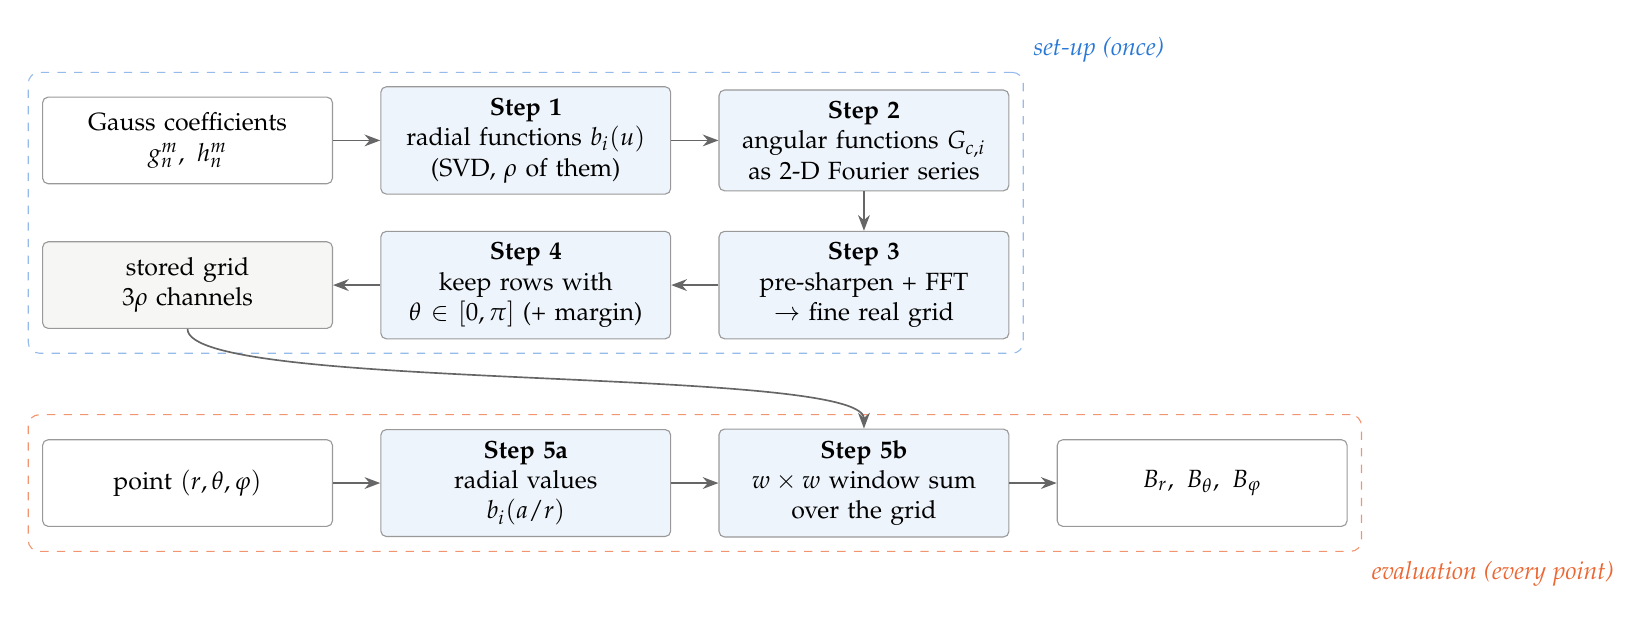
\begin{tikzpicture}[node distance=5mm and 6mm, font=\small,
  box/.style={draw=black!40, rounded corners=2pt, fill=white, align=center, inner sep=4pt, text width=34mm, minimum height=11mm},
  pbox/.style={box, fill=boxbg},
  arr/.style={-{Stealth[length=2mm]}, black!60, line width=0.6pt}]
\node[box] (coef) {Gauss coefficients\\$g_n^m,\ h_n^m$};
\node[pbox, right=of coef] (s1) {\textbf{Step 1}\\radial functions $b_i(u)$\\(SVD, $\rho$ of them)};
\node[pbox, right=of s1] (s2) {\textbf{Step 2}\\angular functions $G_{c,i}$\\as 2-D Fourier series};
\node[pbox, below=of s2] (s3) {\textbf{Step 3}\\pre-sharpen + FFT\\$\to$ fine real grid};
\node[pbox, left=of s3] (s4) {\textbf{Step 4}\\keep rows with\\$\theta\in[0,\pi]$ (+ margin)};
\node[box, left=of s4, fill=codebg] (grid) {stored grid\\$3\rho$ channels};
\begin{scope}[on background layer]
\node[draw=accent!50, dashed, rounded corners, fit=(coef)(s1)(s2)(s3)(s4)(grid), inner sep=5pt, label={[font=\small\itshape, text=accent]north east:set-up (once)}] {};
\end{scope}
\node[box, below=14mm of grid] (pt) {point $(r,\theta,\varphi)$};
\node[pbox, right=of pt] (s5a) {\textbf{Step 5a}\\radial values\\$b_i(a/r)$};
\node[pbox, right=of s5a] (s5b) {\textbf{Step 5b}\\$w\times w$ window sum\\over the grid};
\node[box, right=of s5b] (out) {$B_r,\ B_\theta,\ B_\varphi$};
\begin{scope}[on background layer]
\node[draw=C2orange!70, dashed, rounded corners, fit=(pt)(s5a)(s5b)(out), inner sep=5pt, label={[font=\small\itshape, text=C2orange]south east:evaluation (every point)}] {};
\end{scope}
\draw[arr] (coef)--(s1); \draw[arr] (s1)--(s2); \draw[arr] (s2)--(s3); \draw[arr] (s3)--(s4); \draw[arr] (s4)--(grid);
\draw[arr] (pt)--(s5a); \draw[arr] (s5a)--(s5b); \draw[arr] (s5b)--(out);
\draw[arr] (grid.south) .. controls +(0,-8mm) and +(0,8mm) .. (s5b.north);
\end{tikzpicture}}
\caption{Structure of the method. Everything in the upper box depends only on the model and is done once. Each point
then needs only Step 5.}
\label{fig:pipeline}
\end{figure}

\keyidea{\textbf{Key idea.} After the set-up, the model has become a table of numbers on a regular grid. Each evaluation
reads a small, fixed-size patch of that table. Its cost does not depend on $L$, which is where the speed comes from.}

%=====================================================================
\section{Step 1: separating the radial dependence}\label{sec:step1}
%=====================================================================

\subsection{The radial factors}
In~\eqref{eq:shape}, the radius enters only through the powers $u^{n+2}$, with a different power for every degree $n$. A satellite data
set covers a shell $r_{\min}\le r\le r_{\max}$, for example 250--800\,km altitude. So $u=a/r$ lies in an interval
$[u_0,u_1]$ with $u_0=a/r_{\max}$ and $u_1=a/r_{\min}$. For the 250--800\,km shell this is $[0.888,0.962]$, a narrow interval.

On a narrow interval, the $L$ functions $u^3,u^4,\dots,u^{L+2}$ look very much alike: they are all smooth, increasing
curves. Intuitively, they can be built from a few ``shape'' functions. That is exactly what the singular value decomposition (SVD) finds.

\subsection{Low rank and the SVD}
Suppose we can find $\rho$ functions $b_1(u),\dots,b_\rho(u)$ and numbers $\beta_{i,n}$ with
\begin{equation}\label{eq:radsplit}
u^{n+2}\approx\sum_{i=1}^{\rho}\beta_{i,n}\,b_i(u)\qquad\text{for all }u\in[u_0,u_1]\text{ and all }n=1,\dots,L.
\end{equation}
Substituting into~\eqref{eq:shape} and swapping the order of the sums gives
\begin{equation}\label{eq:BG}
\boxed{\;B_c(r,\theta,\varphi)=\sum_{i=1}^{\rho}b_i(u)\;G_{c,i}(\theta,\varphi),\qquad
G_{c,i}(\theta,\varphi)=\Re\sum_{n,m}\beta_{i,n}\,\gamma_n^m\,\Theta_c^{nm}(\theta)\,e^{\ii m\varphi}.\;}
\end{equation}
The radius now appears only in the $\rho$ numbers $b_i(u)$. The angular functions $G_{c,i}$ do not depend on $r$ at all. If $\rho$ is small,
we have turned a 3-D problem into $\rho$ two-dimensional ones.

To find the best $b_i$, sample the functions at $K+1$ points $u_0\le u_j\le u_1$ and put them in a matrix
\begin{equation}
A_{jn}=\sqrt{c_j}\;w_n\;u_j^{\,n+2}\qquad(j=0,\dots,K;\ n=1,\dots,L).
\end{equation}
\begin{itemize}
\item Each column of $A$ is one radial function.
\item The weights $w_n=(n+1)\big(\sum_m|\gamma_n^m|^2\big)^{1/2}$ measure how strongly degree $n$ contributes to the field, so the
  approximation is most accurate where it matters.
\item The factors $\sqrt{c_j}$ are quadrature weights explained in \cref{app:radial}.
\end{itemize}
The SVD writes
\begin{equation}
A=U\,S\,W^{\mathsf T}=\sum_{i}s_i\,\mathbf u_i\,\mathbf w_i^{\mathsf T},\qquad s_1\ge s_2\ge\dots\ge0,
\end{equation}
where the columns $\mathbf u_i$ of $U$ and $\mathbf w_i$ of $W$ are orthonormal. Keeping only the first $\rho$ terms gives the best approximation of $A$
by a matrix of rank $\rho$ (the Eckart--Young theorem~\cite{golub2013}). The error is governed by the first omitted singular
value $s_{\rho+1}$. We choose $\rho$ as the number of singular values with $s_i>\tau\,s_1$, where $\tau$ is a small multiple of the target accuracy.
Reading off the columns gives $b_i(u_j)=U_{ji}/\sqrt{c_j}$ and $\beta_{i,n}=s_iW_{ni}/w_n$.

\begin{figure}[!htbp]\centering
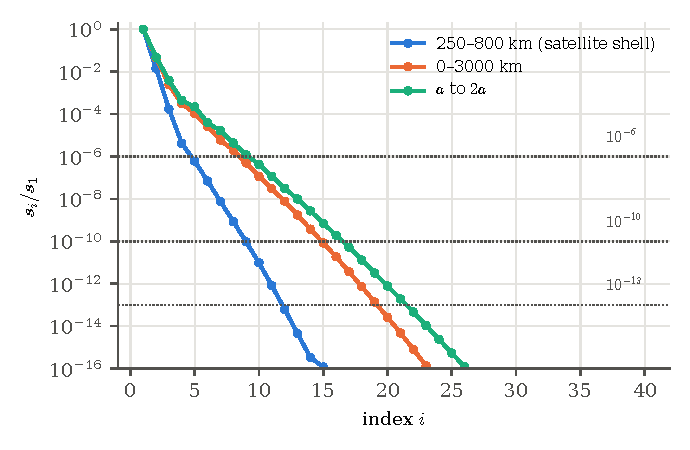
\includegraphics[width=.62\linewidth]{fig/singular.pdf}
\caption{Singular values $s_i/s_1$ of the weighted radial functions for $L=185$. For the satellite shell (blue) they fall
below $10^{-6}$ after 5 terms and below $10^{-13}$ after about 13. Thicker shells need more terms (orange, green).}
\label{fig:singular}
\end{figure}

\Cref{fig:singular} shows why this works so well. For the satellite shell the singular values fall extremely fast:
about 5 radial functions suffice for an accuracy of $10^{-6}$ and about 12 for $10^{-13}$, although there are 185 different powers
$u^{n+2}$. For thicker shells more terms are needed, because the curves $u^{n+2}$ differ more over a wider interval.

\subsection{Building the basis in practice}
\begin{itemize}
\item \textbf{Sample points.} We use Chebyshev points: $u_j=u_c+u_d\cos(\pi j/K)$, with $u_c=\tfrac12(u_0+u_1)$ and
  $u_d=\tfrac12(u_1-u_0)$. On these points, smooth functions can be represented by Chebyshev series that converge very
  fast (\cref{app:radial}). The number of points $K+1$ is increased until the functions are resolved to the target
  accuracy; typically $K=6$--$20$.
\item \textbf{Evaluating $b_i$ at an arbitrary radius.} Each basis function is stored as a short Chebyshev series in $t=(u-u_c)/u_d\in[-1,1]$,
  $b_i(u)=\sum_{k=0}^{K}C_{ik}T_k(t)$. The Chebyshev polynomials satisfy $T_0=1$, $T_1=t$ and $T_{k+1}=2tT_k-T_{k-1}$, so
  computing all $\rho$ values at a point costs about $\rho K$ operations.
\end{itemize}

%=====================================================================
\section{Step 2: the angular functions as Fourier series}\label{sec:step2}
%=====================================================================

Each angular function in~\eqref{eq:BG} is a sum of products of a function of $\theta$ and $e^{\ii m\varphi}$.
The $\varphi$ part is already a Fourier series. This section shows that the $\theta$ part is one too, with one extra trick.

\subsection{The doubled sphere}
Colatitude only runs from $0$ to $\pi$, so functions of $\theta$ are not naturally periodic. The trick is to let
$\theta$ run over a full circle, $[0,2\pi)$, and to evaluate $\cos\theta$ and $\sin\theta$ there as usual. Then
$\sin\theta$ is negative on $(\pi,2\pi)$. This is called the \emph{doubled sphere}: the second half is a mirror
image of the first, as \cref{fig:doubled} shows. The same device underlies the fast spherical Fourier transforms of Kunis and Potts~\cite{kunis2003}. Points of the Earth only ever have $\theta\in[0,\pi]$, but the extended
functions are periodic, and that is what Fourier series need.

\begin{figure}[!htbp]\centering
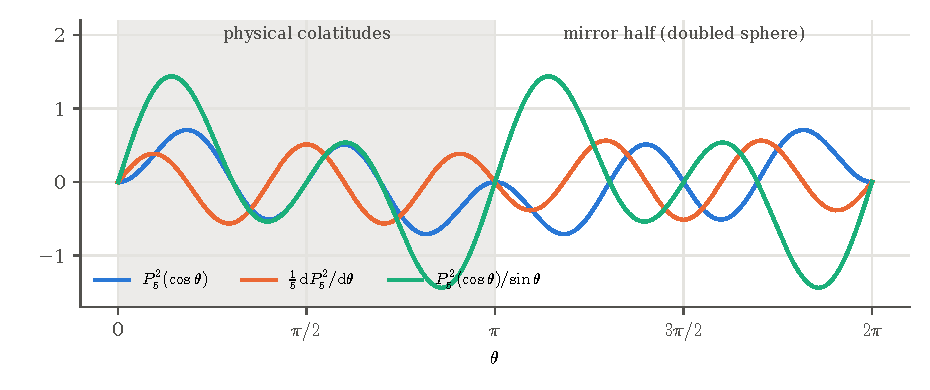
\includegraphics[width=.86\linewidth]{fig/doubled.pdf}
\caption{Legendre functions continued to the doubled sphere $\theta\in[0,2\pi)$, here for $n=5$, $m=2$. All three
functions are smooth and $2\pi$-periodic, including at the poles $\theta=0$ and $\theta=\pi$. The quotient $P/\sin\theta$ is regular
even though $\sin\theta=0$ at the poles.}
\label{fig:doubled}
\end{figure}

\subsection{Legendre functions are trigonometric polynomials}
\begin{lemma}\label{lem:legendre}
On the doubled sphere, $P_n^m(\cos\theta)$ and $\dd P_n^m/\dd\theta$ are trigonometric polynomials of degree at most $n$.
For $m\ge1$, $P_n^m(\cos\theta)/\sin\theta$ is a trigonometric polynomial of degree at most $n-1$.
\end{lemma}
\begin{proof}
From its definition, $P_n^m(\cos\theta)=c\,\sin^m\theta\;q(\cos\theta)$, where $q$ is an ordinary polynomial of degree $n-m$ and $c$ a constant. Each product
$\sin^m\theta\cos^j\theta$ with $j\le n-m$ can be expanded, using $\sin\theta=(e^{\ii\theta}-e^{-\ii\theta})/(2\ii)$ and
$\cos\theta=(e^{\ii\theta}+e^{-\ii\theta})/2$, into powers $e^{\ii p\theta}$ with $|p|\le m+j\le n$. Differentiating
$e^{\ii p\theta}$ gives $\ii p\,e^{\ii p\theta}$, so the derivative has the same degree. Finally, for $m\ge1$,
$P_n^m/\sin\theta=c\,\sin^{m-1}\theta\,q(\cos\theta)$ has degree at most $n-1$.
\end{proof}
Two consequences matter.
\begin{itemize}
\item \textbf{No pole problem.} The factor $1/\sin\theta$ in $B_\varphi$ is cancelled exactly. Our recursions compute
  $P_n^m/\sin\theta$ directly, without ever dividing by $\sin\theta$ (\cref{app:recursions}).
\item \textbf{Exact Fourier series.} Every angular function is an exact 2-D trigonometric polynomial of degree at most $L$ in both $\theta$ and $\varphi$:
\begin{equation}\label{eq:Gfourier}
G_{c,i}(\theta,\varphi)=\Re\sum_{p=-L}^{L}\sum_{m=0}^{L}H_{c,i}[p,m]\,e^{\ii(p\theta+m\varphi)},\qquad
H_{c,i}[p,m]=\sum_{n=\max(m,1)}^{L}\beta_{i,n}\,\gamma_n^m\,\widehat{\Theta}_c^{nm}[p],
\end{equation}
where $\widehat{\Theta}_c^{nm}[p]$ are the Fourier coefficients of $\Theta_c^{nm}(\theta)$.
\end{itemize}

\subsection{Computing the coefficients exactly}
By \cref{lem:sampling}, the Fourier coefficients of a degree-$L$ function are obtained \emph{exactly} from $2L+2$ equally
spaced samples. We sample at $\theta_j=(j+\tfrac12)\,2\pi/(2L+2)$; the half-step shift keeps the samples off the poles, which is
harmless and slightly tidier. For each order $m$:
\begin{enumerate}
\item compute $P_n^m$, $\dd P_n^m/\dd\theta$ and $P_n^m/\sin\theta$ at all $\theta_j$ for $n=m,\dots,L$, using the recursions;
\item take one FFT of each row to get $\widehat\Theta_c^{nm}[p]$ for $|p|\le L$;
\item form $H_{c,i}[\,\cdot\,,m]$ by the sum over $n$ in~\eqref{eq:Gfourier}, which is a small matrix product.
\end{enumerate}
No approximation is made in this step.

\subsection{Making the functions real}\label{sec:real}
The functions $G_{c,i}$ are real, but~\eqref{eq:Gfourier} writes them as the real part of a complex series that uses
only $m\ge0$. For the next step it is simpler and faster to write them as an ordinary two-sided series with real values:
\begin{equation}\label{eq:Freal}
G_{c,i}(\theta,\varphi)=\sum_{p=-L}^{L}\sum_{m=-L}^{L}F_{c,i}[p,m]\,e^{\ii(p\theta+m\varphi)} .
\end{equation}
Using $\Re z=\tfrac12(z+\bar z)$, the new coefficients are
\begin{align}
F[p,m]&=\tfrac12H[p,m],\qquad F[p,-m]=\tfrac12\overline{H[-p,m]}\qquad(m>0),\\
F[p,0]&=\tfrac12\big(H[p,0]+\overline{H[-p,0]}\big).
\end{align}
They satisfy $F[-p,-m]=\overline{F[p,m]}$, which is exactly the condition for the sum to be real. The gain shows up in
Step 3: the grid then holds real numbers instead of complex ones, and evaluation needs no extra phase factor.

%=====================================================================
\section{Step 3: pre-sharpening and the fine grid}\label{sec:step3}
%=====================================================================

We now face the central question: given a Fourier series, how do we evaluate it quickly at many \emph{arbitrary}
points? We explain the idea in one dimension first, then extend it to two.

\subsection{The one-dimensional problem}
Let $f(x)=\sum_{|k|\le N}c_ke^{\ii kx}$. Evaluating it directly at one point costs $2N+1$ operations. We want something cheaper
when there are many points.

\paragraph{First attempt: sample and interpolate.} Use the FFT to compute $f$ on a fine grid $x_l=lh$ with
$h=2\pi/n_f$. Then estimate $f(x)$ from nearby grid values, as one would interpolate in a table. With a few
neighbours, ordinary (e.g.\ polynomial) interpolation is not very accurate. The \emph{exact} formula for reconstructing a
trigonometric polynomial from its samples does exist, but its kernel, the Dirichlet kernel, decays slowly, so every grid value
contributes. That is no cheaper than the direct sum.

\paragraph{The trick: change what we store.} Choose a smooth \emph{window} function $\phi(x)$ that is zero outside a short
interval of width $wh$, i.e.\ $w$ grid steps. Store on the grid, not the samples $f(x_l)$, but the \emph{pre-sharpened}
values
\begin{equation}\label{eq:bl}
b_l=\sum_{k=-N}^{N}c_k\,\frac{h}{\hat\phi(k)}\,e^{\ii kx_l},\qquad
\hat\phi(k)=\int_{-\infty}^{\infty}\phi(x)\,e^{-\ii kx}\,\dd x ,
\end{equation}
where $\hat\phi$ is the Fourier transform of the window. This is again an FFT, of the modified coefficients
$c_kh/\hat\phi(k)$. Then evaluate
\begin{equation}\label{eq:recon}
\tilde f(x)=\sum_{l}b_l\,\phi(x-x_l),
\end{equation}
which involves only the $w$ grid points within the window around $x$.

\paragraph{Why it works.} The Poisson summation formula states that summing a function over a regular grid equals
summing its Fourier transform over the ``reciprocal'' grid: $\sum_lg(lh)=\frac1h\sum_j\hat g(2\pi j/h)$. Applying it to
$g(y)=\phi(x-y)e^{\ii ky}$ gives the identity
\begin{equation}\label{eq:poisson}
\sum_{l}\phi(x-x_l)\,e^{\ii kx_l}=\frac1h\sum_{j=-\infty}^{\infty}\hat\phi(k-jn_f)\,e^{\ii(k-jn_f)x}.
\end{equation}
Inserting~\eqref{eq:bl} into~\eqref{eq:recon} and using~\eqref{eq:poisson} gives
\begin{equation}\label{eq:error}
\tilde f(x)=f(x)+\underbrace{\sum_{k}c_k\sum_{j\ne0}\frac{\hat\phi(k-jn_f)}{\hat\phi(k)}\,e^{\ii(k-jn_f)x}}_{\text{error}} .
\end{equation}
The $j=0$ term reproduces $f$ exactly, because the factor $h/\hat\phi(k)$ in $b_l$ cancels the factor $\hat\phi(k)/h$ produced by the
window sum. That is the purpose of pre-sharpening. The remaining terms are copies of the spectrum shifted by multiples of $n_f$: the aliases.

\keyidea{\textbf{Pre-sharpening in one sentence.} Dividing each Fourier coefficient by $\hat\phi(k)$ before going to the grid
undoes, in advance, the blurring that the short window sum will cause. What is left is an error made only of aliases, and
these can be made as small as we like.}

\subsection{Why the error is tiny: oversampling}\label{sec:oversampling}
The error in~\eqref{eq:error} is small if $\hat\phi$ is large on the band $|k|\le N$ and tiny at the alias frequencies $|k-jn_f|\ge n_f-N$.
\begin{itemize}
\item \textbf{Oversampling.} We make the grid finer than \cref{lem:sampling} requires, $n_f=\sigma(2N+1)$ with an
  \emph{oversampling factor} $\sigma=2$. This leaves a gap between the band and the nearest alias (\cref{fig:window}, right).
\item \textbf{A window with a sharp spectrum.} A window that is short in space cannot have a perfectly sharp spectrum (an
  uncertainty principle), but some windows come close. We use the ``exponential of semicircle''
  window~\cite{barnett2019}:
\begin{equation}\label{eq:es}
\phi(x)=\exp\!\Big(\beta\big(\sqrt{1-z^2}-1\big)\Big),\qquad z=\frac{x}{wh/2},\quad |z|\le1,
\end{equation}
and $\phi=0$ for $|z|>1$. Its spectrum is nearly flat and then drops by a large factor at frequency $\approx\beta n_f/(\pi w)$.
\item \textbf{Placing the drop.} We choose $\beta=\pi(1-\tfrac1{2\sigma})\,w$, so that the drop sits exactly at the nearest alias $n_f-N$.
  The ratio $\hat\phi(k-jn_f)/\hat\phi(k)$ is then of order $e^{-\beta}$, i.e.\ roughly $10^{-w}$ for $\sigma=2$.
\end{itemize}
\textbf{Each extra grid point in the window buys about one more correct digit}, as the measurements in \cref{sec:accuracy} confirm.

\begin{figure}[!htbp]\centering
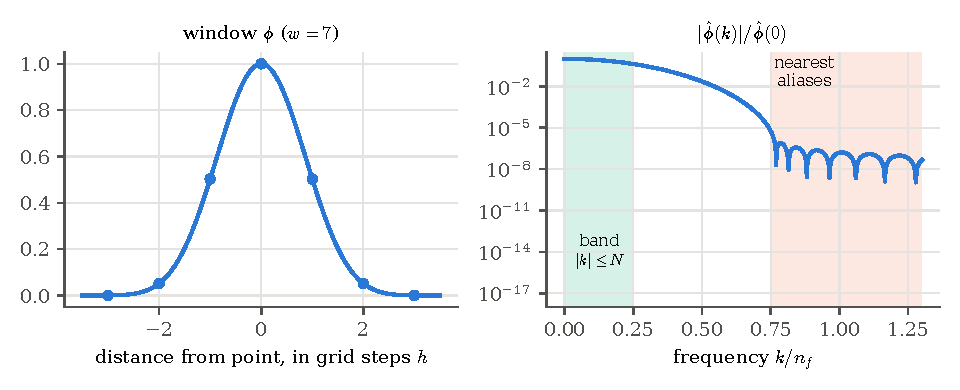
\includegraphics[width=.9\linewidth]{fig/window.pdf}
\caption{\emph{Left:} the window~\eqref{eq:es} for $w=7$, with the 7 grid points it touches (dots). \emph{Right:} its spectrum.
It is nearly constant on the band of the function (green), and seven orders of magnitude smaller at the aliases (orange).
That ratio is the error of the method.}
\label{fig:window}
\end{figure}

\begin{example}[One dimension]
\Cref{fig:presharp} takes a random real trigonometric polynomial of degree $N=10$, on a grid of $n_f=42$ points ($\sigma=2$).
The pre-sharpened values $b_l$ (squares) differ visibly from plain samples (circles); they are not samples of $f$. Yet the
7-point window sum~\eqref{eq:recon} reproduces $f$ everywhere with an error of about $10^{-6}$. With 10 points the error is
$10^{-9}$; with 4 points it is $10^{-3}$.
\end{example}

\begin{figure}[!htbp]\centering
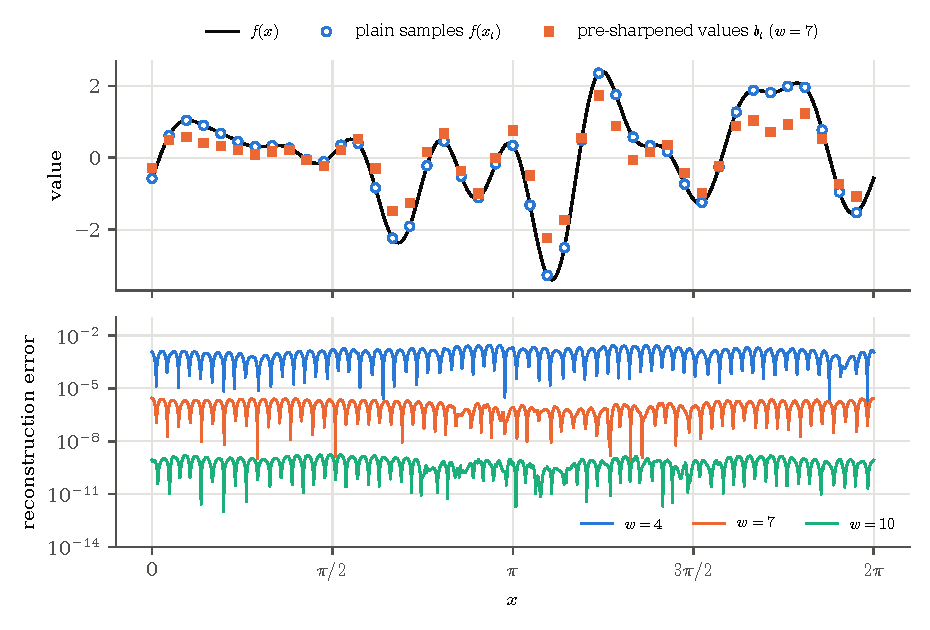
\includegraphics[width=.88\linewidth]{fig/presharp.pdf}
\caption{Pre-sharpening in one dimension. \emph{Top:} a trigonometric polynomial, its plain samples and the pre-sharpened grid
values for $w=7$. \emph{Bottom:} error of the window reconstruction~\eqref{eq:recon} at 1500 points, for three window widths.}
\label{fig:presharp}
\end{figure}

\subsection{From one dimension to two}
In two dimensions we use the product window $\phi(\theta)\,\phi(\varphi)$, whose Fourier transform is also a product. Everything above carries over:
\begin{enumerate}
\item multiply each coefficient $F_{c,i}[p,m]$ of~\eqref{eq:Freal} by $\dfrac{h_1}{\hat\phi_1(p)}\cdot\dfrac{h_2}{\hat\phi_2(m)}$ (pre-sharpening);
\item place the result in an $n_{f,1}\times n_{f,2}$ array of frequencies, with $n_{f,d}\approx\sigma(2L+1)$, and apply a 2-D inverse
  FFT. Because the coefficients have the Hermitian symmetry of \cref{sec:real}, the result is a real grid $g_{c,i}[l_1,l_2]$;
\item a point $(\theta,\varphi)$ is then evaluated as $\sum_{l_1,l_2}g_{c,i}[l_1,l_2]\,\phi(\theta-l_1h_1)\,\phi(\varphi-l_2h_2)$, which involves
  only $w\times w$ grid values.
\end{enumerate}
The set-up performs one such FFT for each of the $3\rho$ ``channels'' $(c,i)$: three field components times $\rho$ radial
functions. This is the only place where FFTs are used, and they are done once.

\subsection{Step 3 is a NUFFT}\label{sec:nufft}
Pre-sharpening, FFT and window sum are exactly the three stages of a \emph{type-2 non-uniform FFT} (NUFFT)~\cite{dutt1993,greengard2004,barnett2019},
the standard tool for evaluating Fourier series at scattered points. The only difference from a textbook NUFFT is the order of work. A NUFFT library
normally receives new Fourier coefficients on every call, so it repeats the pre-sharpening and FFT each time. Our coefficients are fixed by the model, so
these two stages are done once, in the set-up, and only the window sum is repeated for each batch of points.

\paragraph{Why a purpose-built window sum?} General NUFFT libraries such as FINUFFT~\cite{barnett2019} are designed for ``one grid, many points''.
Our problem is ``$3\rho$ grids, the same points, combined at the end''. A library can be used, and we provide this as an option (\cref{sec:step5}),
but it treats each grid as a separate transform: it recomputes every point's window weights for each grid, and returns per-grid results that must be
read back for the radial sum. Step~5 instead uses a loop written for this structure: the window weights are computed once per point, and all grids
are summed in one pass together with the radial combination. Measured, this is about $1.4\times$ faster (\cref{tab:backends}).

\paragraph{Using FINUFFT's window instead.} When the library is used, the pre-sharpening factors must match \emph{its} window exactly. We obtain them by
asking the library itself: we place a pure Fourier mode $e^{\ii kx}$ on the grid and let FINUFFT interpolate it at a few points. The result is
$r_k\,e^{\ii kx}$, apart from aliases of size $\approx\eps$, where $r_k$ is precisely the factor by which the window sum scales frequency $k$. Dividing
every Fourier coefficient by $r_k$ (instead of by $\hat\phi(k)/h$) makes the library's window sum reproduce the series, without any knowledge of its
internal formulas.

%=====================================================================
\section{Step 4: storing only what is needed}\label{sec:half}\label{sec:step4}
%=====================================================================

The grid covers the whole doubled sphere, $\theta\in[0,2\pi)$, but real points have $\theta\in[0,\pi]$. A point's window
reaches at most $w/2$ grid steps on either side. So the only rows that can ever be read are those with
\begin{equation}
-\tfrac w2h_1\;\lesssim\;\theta_{l_1}\;\lesssim\;\pi+\tfrac w2h_1 .
\end{equation}
We store just these rows, about half of the grid plus a margin of $w$ rows (\cref{fig:band}). The margin rows below
$\theta=0$ and above $\theta=\pi$ hold values from the mirror half of the doubled sphere. They are needed by points close to a pole,
whose window straddles the pole. Because the angular functions are smooth trigonometric polynomials across the poles (\cref{lem:legendre}),
the window sum is just as accurate there as anywhere else.

\begin{figure}[!htbp]\centering
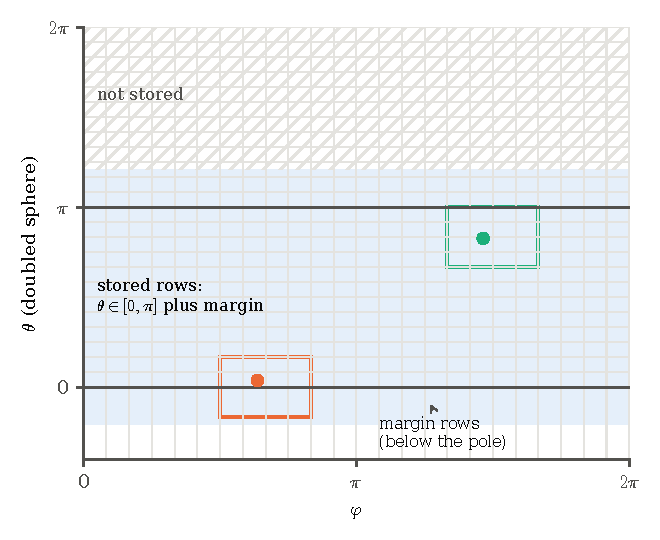
\includegraphics[width=.55\linewidth]{fig/band.pdf}
\caption{The grid on the doubled sphere. Only the shaded rows are stored. Boxes show the $w\times w$ windows of two points. The window of
the point near the North pole reaches into the margin rows below $\theta=0$.}
\label{fig:band}
\end{figure}

This halves the memory. The real-valued grid of \cref{sec:real} has the same size as the earlier complex one (twice as many columns, half the bytes
per value), so the net effect is a factor of two: for $L=185$, $w=14$ and $\rho=14$ the stored grid shrinks from 190\,MB to 98\,MB (\cref{tab:oldnew}).

%=====================================================================
\section{Step 5: evaluating at the points}\label{sec:step5}
%=====================================================================

For a point $(r,\theta,\varphi)$ the evaluation does the following.
\begin{enumerate}
\item \textbf{Window weights.} Find the first grid row and column of the window,
  $\ell_1=\lceil\theta/h_1-w/2\rceil$ and $\ell_2=\lceil\varphi/h_2-w/2\rceil$, and compute the $w$ weights
  $\phi(\theta-(\ell_1+a)h_1)$ and the $w$ weights $\phi(\varphi-(\ell_2+b)h_2)$, for $a,b=0,\dots,w-1$. This takes $2w$ exponentials.
\item \textbf{Window sum, all channels at once.} The grid is stored so that the $3\rho$ channel values of one grid node are next to each
  other in memory. One pass over the $w\times w$ nodes accumulates
\begin{equation}
s_{c,i}=\sum_{a,b=0}^{w-1}\phi_1[a]\,\phi_2[b]\;g_{c,i}[\ell_1+a,\ \ell_2+b]
\end{equation}
  for all channels together (column indices are taken modulo $n_{f,2}$, since $\varphi$ is periodic). This is the main cost: $3\rho\,w^2$ multiply--adds.
\item \textbf{Radial values.} With $t=(a/r-u_c)/u_d$, compute $T_0(t),\dots,T_K(t)$ by recurrence and $b_i=\sum_kC_{ik}T_k(t)$.
\item \textbf{Combine.} $B_c=\sum_{i=1}^{\rho}b_i\,s_{c,i}$ for $c=r,\theta,\varphi$.
\end{enumerate}
\paragraph{Two implementations of the window sum.} The code offers two ways to carry out item~2.
\begin{itemize}
\item \textbf{Own fused loop (default).} A compiled loop that, for each point, computes the window weights once and sweeps all $3\rho$ channels
  together, followed directly by the radial sum. Points are first sorted into small blocks of the grid (a counting sort, $\Oh(M)$) so that
  consecutive points read nearby memory, and blocks of points are processed in parallel on all CPU cores. Because the per-point work is done once
  and no intermediate results leave the processor's caches, it is about $1.4\times$ faster than the library (\cref{tab:backends}).
\item \textbf{FINUFFT (optional).} The stored grid is passed to FINUFFT's interpolation-only mode as a batch of transforms that share the same
  points. Since the window weights are real, two real channels are packed into one complex grid, $g_{\text{pair}}=g_{c,i}+\ii\,g_{c',i'}$: the real part of the
  result belongs to the first channel and the imaginary part to the second. This halves the number of transforms to $\lceil3\rho/2\rceil$. The library
  sorts the points for good memory access, evaluates its window with vectorised code and uses all CPU cores. The stored band of rows is passed as a
  grid of its own, with the colatitude coordinate shifted and rescaled so that one library grid step equals one row, and with two extra margin rows
  on each side.
\end{itemize}

%=====================================================================
\section{The complete algorithm}\label{sec:algorithm}
%=====================================================================

\begin{algorithm}[!htbp]
\caption{Set-up (once per model and radial range)}\label{alg:setup}
\begin{algorithmic}[1]
\Require Gauss coefficients $g_n^m,h_n^m$ ($n\le L$); reference radius $a$; radial range $[r_{\min},r_{\max}]$; target accuracy $\eps$
\State $u_0\gets a/r_{\max}$, $u_1\gets a/r_{\min}$; \ $\gamma_n^m\gets g_n^m-\ii h_n^m$; \ $w_n\gets(n+1)\|\gamma_n\|$
\State \textbf{Step 1:} sample $w_nu^{n+2}$ at $K+1$ Chebyshev points; SVD; keep $\rho$ terms; store $C_{ik}$ and $\beta_{i,n}$
\State \textbf{Step 2:} $\theta_j\gets(j+\tfrac12)\frac{2\pi}{2L+2}$, $j=0..2L+1$
\For{$m=0,\dots,L$}
  \State $P_n^m,\ \dd P_n^m/\dd\theta,\ P_n^m/\sin\theta$ at all $\theta_j$, $n=m..L$ \Comment{recursions, \cref{app:recursions}}
  \State FFT along $j$ $\to\widehat\Theta_c^{nm}[p]$, $|p|\le L$
  \State $H_{c,i}[p,m]\gets\sum_n\beta_{i,n}\gamma_n^m\widehat\Theta_c^{nm}[p]$ \Comment{three small matrix products}
\EndFor
\State choose $w$ from $\eps$ (\cref{tab:calib}); $\sigma\gets2$; $\beta\gets\pi(1-\tfrac1{2\sigma})w$; $n_{f,d}\gtrsim\sigma(2L+1)$
\For{each channel $(c,i)$}
  \State $F\gets$ real two-sided coefficients of $H_{c,i}$ \Comment{\cref{sec:real}}
  \State \textbf{Step 3:} $F[p,m]\gets F[p,m]\cdot h_1h_2/(\hat\phi_1(p)\hat\phi_2(m))$; zero-pad; real 2-D inverse FFT $\to$ grid
  \State \textbf{Step 4:} store rows $\lceil-w/2\rceil\dots\lceil\pi/h_1-w/2\rceil+w-1$ into $g[\,\cdot,\cdot,(c,i)]$
\EndFor
\end{algorithmic}
\end{algorithm}

\begin{algorithm}[!htbp]
\caption{Evaluation at $M$ points (Step 5)}\label{alg:eval}
\begin{algorithmic}[1]
\Require points $(r_j,\theta_j,\varphi_j)$ with $r_j\in[r_{\min},r_{\max}]$
\State sort the points by grid block
\ForAll{points $j$, in parallel}
  \State $\ell_1\gets\lceil\theta_j/h_1-w/2\rceil$, $\ell_2\gets\lceil\varphi_j/h_2-w/2\rceil$; window weights $\phi_1[0..w-1]$, $\phi_2[0..w-1]$
  \State $\mathbf s\gets\mathbf 0\in\mathbb R^{3\rho}$
  \For{$a=0..w-1$} \For{$b=0..w-1$}
    \State $\mathbf s\gets\mathbf s+\phi_1[a]\,\phi_2[b]\;g[\ell_1+a,\ (\ell_2+b)\bmod n_{f,2},\ :\,]$ \Comment{all $3\rho$ channels}
  \EndFor\EndFor
  \State $t\gets(a/r_j-u_c)/u_d$; \ $b_i\gets\sum_kC_{ik}T_k(t)$
  \State $B_{c,j}\gets\sum_ib_i\,s_{c,i}$ for $c=r,\theta,\varphi$
\EndFor
\end{algorithmic}
\end{algorithm}

\paragraph{The method as a product of matrices.} Collecting the coefficients into a vector $\boldsymbol\gamma$, the whole method computes
\begin{equation}\label{eq:factor}
\mathbf B=S\;\mathcal F^{-1}\;D\;\Lambda\;R\;\boldsymbol\gamma ,
\end{equation}
where the factors are:
\begin{itemize}
\item $R$: the radial split (Step 1);
\item $\Lambda$: the Legendre-to-Fourier map (Step 2), which is exact;
\item $D$: the diagonal pre-sharpening;
\item $\mathcal F^{-1}$: the inverse FFT (Step 3);
\item $S$: a sparse matrix holding the window weights and the radial values (Step 5), with $3\rho w^2$ non-zeros per point.
\end{itemize}
Only $S$ and the truncation of $R$ are approximations. Everything to the right of $S$ is applied once in the set-up, so evaluation is a single
sparse matrix--vector product. The transpose of~\eqref{eq:factor}, needed when fitting a model to data by least squares, has the same structure.

%=====================================================================
\section{Choosing the parameters}\label{sec:parameters}
%=====================================================================

The user chooses the target relative accuracy $\eps$ and the radial range. Everything else follows:
\begin{itemize}
\item \textbf{Window width $w$:} the smallest $w$ whose \emph{measured} error is below $\eps$ (\cref{tab:calib}): $w=7$ for $\eps=10^{-6}$, $11$ for
  $10^{-10}$ and $14$ for $10^{-13}$. (With the optional FINUFFT backend, $\eps$ is passed to the library, which chooses the same widths.) The measured error is practically the same for $L=13$ and $L=185$, so one table serves all models.
\item \textbf{Oversampling $\sigma=2$.} A larger $\sigma$ allows a slightly smaller $w$ for the same accuracy, but makes the stored grid
  larger in proportion to $\sigma^2$. With $\sigma=2$, machine precision is already reached at $w=14$.
\item \textbf{Radial rank $\rho$:} from the SVD, keeping singular values above $0.1\eps$ (\cref{fig:singular}).
\item \textbf{Radial range:} must contain all evaluation points; the code refuses points outside it. A tighter range gives a smaller $\rho$ and
  therefore a faster evaluation.
\end{itemize}

\begin{table}[!htbp]\centering\small
\caption{Measured maximum relative error of the complete transform as a function of the window width $w$
(worst case of $L=13$ and $L=185$, 1500 points including both poles, radial rank at full precision).
The code picks the smallest $w$ whose $\sigma=2$ error is below the requested $\varepsilon$.
For comparison, the direct double-precision sum has error $1.6\times10^{-14}$ at $L=185$.}\label{tab:calib}
\begin{tabular}{rcc}\toprule
$w$&$\sigma=2$ (default)&$\sigma=3$\\\midrule
4 & $7\times10^{-4}$ & $1\times10^{-4}$\\
5 & $2\times10^{-5}$ & $3\times10^{-5}$\\
6 & $4\times10^{-6}$ & $7\times10^{-7}$\\
7 & $6\times10^{-7}$ & $1\times10^{-7}$\\
8 & $3\times10^{-8}$ & $8\times10^{-9}$\\
9 & $4\times10^{-9}$ & $6\times10^{-10}$\\
10 & $6\times10^{-10}$ & $4\times10^{-11}$\\
11 & $3\times10^{-11}$ & $3\times10^{-12}$\\
12 & $3\times10^{-12}$ & $3\times10^{-13}$\\
13 & $5\times10^{-13}$ & $1\times10^{-14}$\\
14 & $4\times10^{-14}$ & --\\
15 & $2\times10^{-14}$ & --\\
\bottomrule\end{tabular}\end{table}


%=====================================================================
\section{Cost and memory}\label{sec:cost}
%=====================================================================

\paragraph{Set-up.}
\begin{itemize}
\item Legendre functions on $2L+2$ sample points for all $(n,m)$: about $L^3$ operations.
\item FFTs in $\theta$: about $L^3\log L$.
\item Matrix products of Step 2: about $3\rho L^3$.
\item $3\rho$ two-dimensional FFTs of size $n_{f,1}\times n_{f,2}\approx(2\sigma L)^2$: about $\rho L^2\log L$.
\end{itemize}
In practice this takes 0.01\,s for $L=13$ and about 1\,s for $L=185$ (\cref{tab:setup}).

\paragraph{Memory.} The stored grid has $3\rho$ channels of about $\tfrac12n_{f,1}\times n_{f,2}\approx2\sigma^2L^2$ real numbers each,
i.e.\ about $3\rho\cdot8L^2\cdot8$ bytes for $\sigma=2$. For $L=185$ that is 34\,MB at $\eps=10^{-6}$ and 84\,MB at machine precision.

\paragraph{Evaluation, per point.}
\begin{itemize}
\item $2w$ window-weight evaluations;
\item $3\rho\,w^2$ multiply--adds for the window sum (the dominant term);
\item about $\rho K$ operations for the radial values.
\end{itemize}
For $\eps=10^{-10}$ ($w=11$, $\rho\approx9$) the window sum is about 3\,300 multiply--adds. \textbf{None of these numbers depends on $L$.}

\paragraph{Comparison with the direct sum.} The direct sum needs about $L^2/2$ terms per point, each costing some 20 operations
(recursions and accumulation): about 340\,000 operations for $L=185$. The fast method therefore wins by a large factor at high
degree. At low degree the two costs become similar. At $\eps=10^{-6}$ the fast method already wins at $L=13$ ($1.4\times$); at $\eps=10^{-10}$ it wins from
$L\approx20$, and at machine precision from $L\approx20$--$30$ (\cref{tab:results}).

\begin{table}[!htbp]\centering\small
\caption{Set-up (precomputation) time in seconds and size of the stored grid in MB.}\label{tab:setup}
\begin{tabular}{r rr rr rr}\toprule
&\multicolumn{2}{c}{$\varepsilon=10^{-6}$}&\multicolumn{2}{c}{$\varepsilon=10^{-10}$}&\multicolumn{2}{c}{$\varepsilon=10^{-13}$}\\
\cmidrule(lr){2-3}\cmidrule(lr){4-5}\cmidrule(lr){6-7}
$L$&set-up&grid&set-up&grid&set-up&grid\\\midrule
13 & 0.01 & 0.2 & 0.01 & 0.3 & 0.01 & 0.4\\
20 & 0.01 & 0.4 & 0.01 & 0.7 & 0.03 & 0.9\\
30 & 0.02 & 0.8 & 0.02 & 1.6 & 0.03 & 2.1\\
45 & 0.03 & 2.3 & 0.05 & 3.4 & 0.06 & 4.5\\
70 & 0.09 & 5.2 & 0.13 & 8.6 & 0.11 & 11\\
100 & 0.22 & 10 & 0.32 & 19 & 0.28 & 23\\
133 & 0.45 & 18 & 0.53 & 33 & 0.49 & 44\\
185 & 0.68 & 34 & 0.95 & 63 & 0.98 & 84\\
\bottomrule\end{tabular}\end{table}


%=====================================================================
\section{Accuracy}\label{sec:accuracy}
%=====================================================================

\paragraph{Error sources.} There are three:
\begin{itemize}
\item the window (the alias terms of~\eqref{eq:error}), controlled by $w$;
\item the truncation of the radial SVD, controlled by $\rho$;
\item floating-point rounding, which is small (\cref{sec:roundoff}).
\end{itemize}
Steps 2 and 3 are otherwise exact.

\paragraph{How we measured it.} To measure errors of order $10^{-14}$ we need a reference that is more accurate than double precision.
We evaluated the model with the same recursions in 80-bit ``long double'' arithmetic, about 19 significant digits, at 1500 random points
in the 250--800\,km shell, including points exactly at both poles. Errors are reported relative to the largest field value,
$\max|\Delta B|/\max|B|$.

\paragraph{Results.} \Cref{fig:calib} and \cref{tab:calib} show the error as a function of $w$. It falls by about a factor of 10 per extra
window point, and is nearly identical for $L=13$ and $L=185$. At $w=14$ it reaches $3$--$4\times10^{-14}$.

\begin{figure}[!htbp]\centering
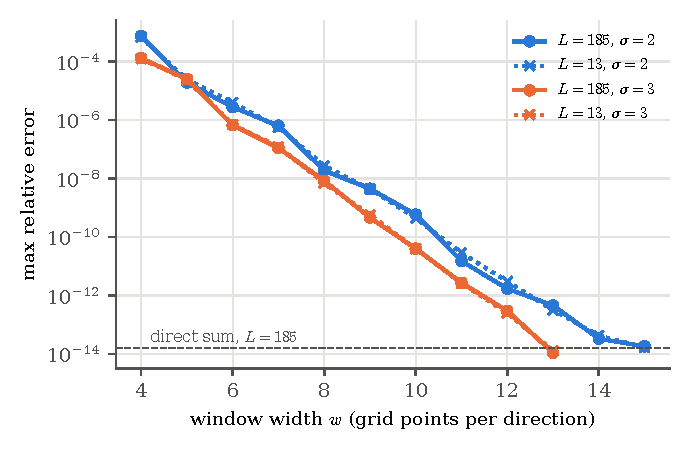
\includegraphics[width=.62\linewidth]{fig/calib.pdf}
\caption{Maximum relative error of the complete transform against the long-double reference, as a function of the window width $w$.
The dashed line is the error of the direct double-precision sum for $L=185$.}
\label{fig:calib}
\end{figure}

\paragraph{Machine precision.}\label{sec:roundoff} The direct sum computed in double precision is not exact either: rounding in its recursions gives
relative errors of $1.1\times10^{-15}$ at $L=13$, growing to $1.6\times10^{-14}$ at $L=185$ ($9\times10^{-10}$\,nT). With $w=14$ the fast method has error
$3.3\times10^{-14}$ at $L=185$, essentially the same. \textbf{At this setting the fast method is as accurate as the direct sum, and still $65\times$ faster} (\cref{tab:results}).

%=====================================================================
\section{Performance results}\label{sec:results}
%=====================================================================

\paragraph{Set-up of the tests.}
\begin{itemize}
\item \textbf{Models.} The IGRF-2025 main field (degrees up to 13, from the IGRF-14 coefficient file). For higher degrees, random
  lithospheric coefficients are added with a CHAOS-like flat spectrum of 0.5\,nT$^2$ per degree at the surface. Speed does not depend on the
  coefficient values.
\item \textbf{Points.} Uniformly random on the sphere, at altitudes between 250 and 800\,km.
\item \textbf{Hardware.} Two CPU cores; both methods use both.
\item \textbf{Timing.} Times are the best of three runs and exclude the set-up unless stated. The direct sum for large $M$ is timed on a subset and scaled, which is
  exact because its cost is proportional to $M$.
\end{itemize}

\paragraph{Findings.} All results are for the default fused loop unless stated; \cref{tab:backends} compares it with the FINUFFT option.
(\Cref{tab:backends} comes from a separate run; repeated runs of the same configuration agree to within a few per cent.)
\begin{itemize}
\item \textbf{FINUFFT option:} the fused loop is 1.1--2.1$\times$ faster than FINUFFT doing the same window sums, typically $1.4\times$; with FINUFFT the
  speedups at $L=185$ are $134\times$, $65\times$ and $43\times$. Both reach the accuracy of the direct sum. At $\eps=10^{-14}$ FINUFFT's tuned window gives
  $4.4\times10^{-15}$ at $L=185$, below the direct sum's own rounding error.
\item \textbf{Cost per point is independent of $L$} (\cref{fig:speed}, right): about 0.3--0.5\,$\mu$s per point at $\eps=10^{-6}$, 0.7--0.9\,$\mu$s at $10^{-10}$
  and 1.1--1.4\,$\mu$s at $10^{-13}$. The direct sum grows from 0.5\,$\mu$s at $L=13$ to 86\,$\mu$s at $L=185$.
\item \textbf{Speedups at $L=185$} with $10^6$ points: $201\times$ ($\eps=10^{-6}$), $98\times$ ($10^{-10}$) and $65\times$ (machine precision).
\item \textbf{IGRF ($L=13$):} the fast method is $1.4\times$ faster at $\eps=10^{-6}$, but slower than the direct sum at higher accuracy. For IGRF alone a good direct
  code remains a sensible choice.
\item \textbf{Including the set-up} (\cref{fig:timeM}), the method breaks even at about $10^4$ points at high degree. At $L=185$ and $10^5$ points it is
  8--12$\times$ faster in total, and 37--78$\times$ faster at $10^6$ points.
\item \textbf{The two simplifications} of \cref{sec:real,sec:half} made evaluation 1.4--1.9$\times$ faster and halved the memory, at identical settings (\cref{tab:oldnew}).
\end{itemize}

\begin{figure}[!htbp]\centering
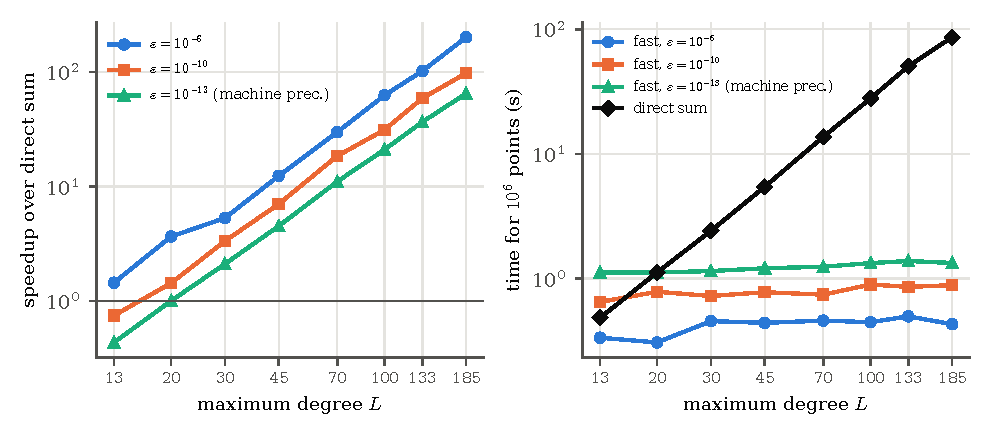
\includegraphics[width=\linewidth]{fig/speed.pdf}
\caption{\emph{Left:} speedup over the direct sum for $10^6$ points. \emph{Right:} time for $10^6$ points. The fast method's cost is flat in $L$,
while the direct sum grows like $L^2$. With the optional FINUFFT backend, times are about $1.4\times$ longer (\cref{tab:backends}).}
\label{fig:speed}
\end{figure}

\begin{figure}[!htbp]\centering
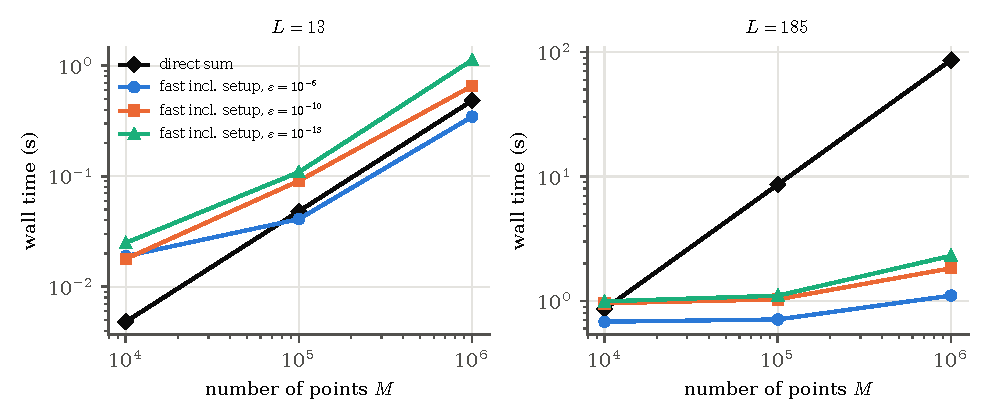
\includegraphics[width=\linewidth]{fig/timeM.pdf}
\caption{Total time \emph{including the set-up} versus the number of points, for IGRF size ($L=13$) and a full lithospheric model ($L=185$).}
\label{fig:timeM}
\end{figure}

\begin{table}[!htbp]\centering\small
\caption{The two implementations of Step 5 at the same requested accuracy $\varepsilon$: FINUFFT's interpolation-only mode (the default)
and our own fused loop. $M=10^6$ points, 250--800\,km shell, two cores. Time in seconds; error is the maximum relative error against the long-double
reference; speedup is relative to the direct sum.}\label{tab:backends}
\begin{tabular}{rr r rrr rrr}\toprule
&&&\multicolumn{3}{c}{FINUFFT (optional)}&\multicolumn{3}{c}{own fused loop (default)}\\
\cmidrule(lr){4-6}\cmidrule(lr){7-9}
$L$&$\varepsilon$&$w$&time&error&speedup&time&error&speedup\\\midrule
13 & $10^{-6}$ & 7 & 0.47 & $9.2\times10^{-7}$ & \textbf{1.0} & 0.33 & $5.6\times10^{-7}$ & 1.5\\
13 & $10^{-10}$ & 11 & 0.97 & $6.8\times10^{-11}$ & \textbf{0.5} & 0.68 & $2.8\times10^{-11}$ & 0.7\\
13 & $10^{-13}$ & 14 & 1.56 & $4.2\times10^{-14}$ & \textbf{0.3} & 1.22 & $4.2\times10^{-14}$ & 0.4\\\addlinespace[2pt]
20 & $10^{-6}$ & 7 & 0.74 & $7.8\times10^{-7}$ & \textbf{1.5} & 0.36 & $6.4\times10^{-7}$ & 3.1\\
20 & $10^{-10}$ & 11 & 1.27 & $7.4\times10^{-11}$ & \textbf{0.9} & 0.74 & $2.3\times10^{-11}$ & 1.5\\
20 & $10^{-13}$ & 14 & 1.46 & $5.7\times10^{-14}$ & \textbf{0.8} & 0.92 & $3.6\times10^{-14}$ & 1.2\\\addlinespace[2pt]
45 & $10^{-6}$ & 7 & 0.61 & $6.2\times10^{-7}$ & \textbf{8.9} & 0.42 & $5.9\times10^{-7}$ & 13\\
45 & $10^{-10}$ & 11 & 1.05 & $6.7\times10^{-11}$ & \textbf{5.2} & 0.99 & $1.3\times10^{-11}$ & 5.5\\
45 & $10^{-13}$ & 14 & 2.53 & $6.1\times10^{-14}$ & \textbf{2.1} & 1.60 & $3.1\times10^{-14}$ & 3.4\\\addlinespace[2pt]
100 & $10^{-6}$ & 7 & 0.67 & $8.1\times10^{-7}$ & \textbf{41} & 0.49 & $6.0\times10^{-7}$ & 57\\
100 & $10^{-10}$ & 11 & 1.28 & $7.4\times10^{-11}$ & \textbf{22} & 0.87 & $1.4\times10^{-11}$ & 32\\
100 & $10^{-13}$ & 14 & 1.96 & $6.8\times10^{-14}$ & \textbf{14} & 1.39 & $3.1\times10^{-14}$ & 20\\\addlinespace[2pt]
185 & $10^{-6}$ & 7 & 0.65 & $1.1\times10^{-6}$ & \textbf{134} & 0.43 & $6.3\times10^{-7}$ & 200\\
185 & $10^{-10}$ & 11 & 1.33 & $8.6\times10^{-11}$ & \textbf{65} & 0.90 & $1.6\times10^{-11}$ & 95\\
185 & $10^{-13}$ & 14 & 2.00 & $5.9\times10^{-14}$ & \textbf{43} & 1.42 & $3.3\times10^{-14}$ & 61\\\addlinespace[2pt]
\bottomrule\end{tabular}\end{table}

\begin{table}[!htbp]\centering\small
\caption{Main results (default fused loop): $M=10^6$ points in the 250--800\,km shell, two CPU cores. Direct sum: time (s) and relative error
against the long-double reference. Fast method, for each requested accuracy $\varepsilon$: window width $w$, radial rank $\rho$, evaluation time (s),
speedup over the direct sum, and measured maximum relative error against the long-double reference.}\label{tab:results}
\begin{tabular}{rrr rrrrrr}\toprule
&\multicolumn{2}{c}{direct sum}&\multicolumn{6}{c}{fast method}\\
\cmidrule(lr){2-3}\cmidrule(lr){4-9}
$L$&time&error&$\varepsilon$&$w$&$\rho$&time&speedup&error\\\midrule
\multirow{3}{*}{13} & \multirow{3}{*}{0.48} & \multirow{3}{*}{$1.1\times10^{-15}$} & $10^{-6}$ & 7 & 4 & 0.33 & \textbf{1.4} & $5.6\times10^{-7}$\\
 & &  & $10^{-10}$ & 11 & 6 & 0.65 & \textbf{0.7} & $2.8\times10^{-11}$\\
 & &  & $10^{-13}$ & 14 & 8 & 1.11 & \textbf{0.4} & $4.2\times10^{-14}$\\\addlinespace[2pt]
\multirow{3}{*}{20} & \multirow{3}{*}{1.12} & \multirow{3}{*}{$1.9\times10^{-15}$} & $10^{-6}$ & 7 & 4 & 0.31 & \textbf{3.7} & $6.4\times10^{-7}$\\
 & &  & $10^{-10}$ & 11 & 7 & 0.78 & \textbf{1.4} & $2.3\times10^{-11}$\\
 & &  & $10^{-13}$ & 14 & 8 & 1.12 & \textbf{1.0} & $3.6\times10^{-14}$\\\addlinespace[2pt]
\multirow{3}{*}{30} & \multirow{3}{*}{2.41} & \multirow{3}{*}{$2.7\times10^{-15}$} & $10^{-6}$ & 7 & 4 & 0.45 & \textbf{5.3} & $6.5\times10^{-7}$\\
 & &  & $10^{-10}$ & 11 & 7 & 0.72 & \textbf{3.3} & $1.5\times10^{-11}$\\
 & &  & $10^{-13}$ & 14 & 9 & 1.15 & \textbf{2.1} & $3.6\times10^{-14}$\\\addlinespace[2pt]
\multirow{3}{*}{45} & \multirow{3}{*}{5.44} & \multirow{3}{*}{$3.8\times10^{-15}$} & $10^{-6}$ & 7 & 5 & 0.44 & \textbf{12} & $5.9\times10^{-7}$\\
 & &  & $10^{-10}$ & 11 & 7 & 0.78 & \textbf{7.0} & $1.3\times10^{-11}$\\
 & &  & $10^{-13}$ & 14 & 9 & 1.21 & \textbf{4.5} & $3.1\times10^{-14}$\\\addlinespace[2pt]
\multirow{3}{*}{70} & \multirow{3}{*}{13.70} & \multirow{3}{*}{$7.1\times10^{-15}$} & $10^{-6}$ & 7 & 5 & 0.46 & \textbf{30} & $6.9\times10^{-7}$\\
 & &  & $10^{-10}$ & 11 & 8 & 0.74 & \textbf{18} & $1.5\times10^{-11}$\\
 & &  & $10^{-13}$ & 14 & 10 & 1.24 & \textbf{11} & $3.3\times10^{-14}$\\\addlinespace[2pt]
\multirow{3}{*}{100} & \multirow{3}{*}{27.89} & \multirow{3}{*}{$8.9\times10^{-15}$} & $10^{-6}$ & 7 & 5 & 0.45 & \textbf{63} & $6.0\times10^{-7}$\\
 & &  & $10^{-10}$ & 11 & 9 & 0.89 & \textbf{31} & $1.4\times10^{-11}$\\
 & &  & $10^{-13}$ & 14 & 11 & 1.33 & \textbf{21} & $3.1\times10^{-14}$\\\addlinespace[2pt]
\multirow{3}{*}{133} & \multirow{3}{*}{50.53} & \multirow{3}{*}{$1.3\times10^{-14}$} & $10^{-6}$ & 7 & 5 & 0.50 & \textbf{102} & $6.1\times10^{-7}$\\
 & &  & $10^{-10}$ & 11 & 9 & 0.86 & \textbf{59} & $1.4\times10^{-11}$\\
 & &  & $10^{-13}$ & 14 & 12 & 1.38 & \textbf{37} & $3.1\times10^{-14}$\\\addlinespace[2pt]
\multirow{3}{*}{185} & \multirow{3}{*}{86.25} & \multirow{3}{*}{$1.6\times10^{-14}$} & $10^{-6}$ & 7 & 5 & 0.43 & \textbf{201} & $6.3\times10^{-7}$\\
 & &  & $10^{-10}$ & 11 & 9 & 0.88 & \textbf{98} & $1.6\times10^{-11}$\\
 & &  & $10^{-13}$ & 14 & 12 & 1.33 & \textbf{65} & $3.3\times10^{-14}$\\\addlinespace[2pt]
\bottomrule\end{tabular}\end{table}

\begin{table}[!htbp]\centering\small
\caption{Effect of the two simplifications of \cref{sec:real,sec:half}: the earlier complex-valued, full-grid implementation (``old'')
versus the real-valued, half-grid implementation (``new''), at identical window width $w$, $\sigma=2$ and radial rank $\rho$.
$M=10^6$ points; times in seconds, grid sizes in MB (0 means below 0.5\,MB).}\label{tab:oldnew}
\begin{tabular}{rrr rrr rr}\toprule
$L$&$w$&$\rho$&old&new&speedup&old grid&new grid\\\midrule
13 & 8 & 5 & 0.64 & 0.41 & 1.56 & 0 & 0\\
13 & 12 & 7 & 1.17 & 0.73 & 1.59 & 1 & 0\\
13 & 14 & 8 & 1.69 & 0.89 & 1.90 & 1 & 0\\
20 & 8 & 5 & 0.60 & 0.44 & 1.36 & 1 & 1\\
20 & 12 & 7 & 1.26 & 0.79 & 1.59 & 1 & 1\\
20 & 14 & 9 & 1.76 & 1.13 & 1.56 & 2 & 1\\
45 & 8 & 6 & 0.83 & 0.51 & 1.63 & 5 & 3\\
45 & 12 & 8 & 1.47 & 0.88 & 1.68 & 7 & 4\\
45 & 14 & 10 & 1.92 & 1.29 & 1.49 & 9 & 5\\
100 & 8 & 7 & 1.01 & 0.53 & 1.91 & 29 & 14\\
100 & 12 & 10 & 1.70 & 1.13 & 1.50 & 41 & 21\\
100 & 14 & 12 & 2.12 & 1.27 & 1.67 & 49 & 25\\
185 & 8 & 7 & 0.96 & 0.51 & 1.87 & 95 & 48\\
185 & 12 & 11 & 1.72 & 1.03 & 1.67 & 149 & 77\\
185 & 14 & 14 & 2.69 & 1.70 & 1.58 & 190 & 98\\
\bottomrule\end{tabular}\end{table}


%=====================================================================
\section{Practical advice and limitations}\label{sec:limits}
%=====================================================================
\begin{itemize}
\item \textbf{When to use it.} Use the method for models of degree $L\gtrsim20$ and more than about $10^4$ points. For IGRF alone the direct
  sum is about as fast.
\item \textbf{Which accuracy.} $\eps=10^{-6}$ corresponds to about 0.04\,nT, well below measurement noise and model uncertainty, and gives the largest
  speedups. Use $\eps=10^{-13}$ when results must match a direct computation to the last digits.
\item \textbf{Radial range.} Set $[r_{\min},r_{\max}]$ as tight as the data allow. Very thick shells need more radial functions; for those, split the data into
  thinner shells, each with its own set-up.
\item \textbf{Time-dependent models.} Coefficients that vary with time, such as IGRF secular variation or the CHAOS core field, can be handled by
  linearity: evaluate one transform per time basis function and combine the results with per-point weights. For CHAOS, the time-dependent
  core field has low degree ($n\le20$) and can simply be evaluated directly. The static lithospheric part, where nearly all of the cost lies, then uses this method.
\item \textbf{Not yet implemented.} The current code does not provide the transpose operation needed for least-squares inversion (structure in \cref{sec:algorithm}),
  the potential $V$ itself, or a GPU version. All are straightforward extensions.
\end{itemize}

%=====================================================================
\section{Summary}
%=====================================================================
A spherical harmonic model can be evaluated at scattered points much faster than by direct summation, by combining four ideas:
\begin{enumerate}
\item \textbf{Low-rank radial structure.} The radial factors $(a/r)^{n+2}$ are captured by a few optimal radial functions found by an SVD.
\item \textbf{Exact Fourier form.} On the doubled sphere, the angular parts are exact 2-D trigonometric polynomials, regular at the poles.
\item \textbf{Pre-sharpening.} Dividing by the window's spectrum and moving to an oversampled grid lets a $w\times w$ window sum reproduce the model, with an error that falls
  by about a factor of ten per window point.
\item \textbf{Economy.} The grid is real-valued and only half of it is stored, and each point is evaluated in one fused pass.
\end{enumerate}
After a set-up of about a second, the cost per point is independent of the degree $L$. At $L=185$ the method is 65--200$\times$ faster than the direct sum,
depending on the accuracy, and it can match the direct sum's own precision.

\appendix
%=====================================================================
\section{Pole-safe recursions for the Legendre functions}\label{app:recursions}
%=====================================================================
Let $x=\cos\theta$ and $s=\sin\theta$; on the doubled sphere $s$ may be negative. Write $Q_n^m=P_n^m/\sin\theta$ for $m\ge1$.

\paragraph{Diagonal ($n=m$).} $P_0^0=1$, $\dd P_0^0/\dd\theta=0$; \ $P_1^1=s$, $\dd P_1^1/\dd\theta=x$, $Q_1^1=1$. For $m\ge2$, with $f_m=\sqrt{(2m-1)/(2m)}$:
\[
P_m^m=f_m\,s\,P_{m-1}^{m-1},\qquad \frac{\dd P_m^m}{\dd\theta}=f_m\Big(s\,\frac{\dd P_{m-1}^{m-1}}{\dd\theta}+x\,P_{m-1}^{m-1}\Big),\qquad Q_m^m=f_m\,s\,Q_{m-1}^{m-1}.
\]
\paragraph{Upward in $n$.} With $A_n^m=\dfrac{2n-1}{\sqrt{n^2-m^2}}$ and $B_n^m=\sqrt{\dfrac{(n-1)^2-m^2}{n^2-m^2}}$ (and the $B$ term omitted for $n=m+1$):
\begin{align*}
P_n^m&=A_n^m\,x\,P_{n-1}^m-B_n^m\,P_{n-2}^m,\\
\frac{\dd P_n^m}{\dd\theta}&=A_n^m\Big(x\,\frac{\dd P_{n-1}^m}{\dd\theta}-s\,P_{n-1}^m\Big)-B_n^m\,\frac{\dd P_{n-2}^m}{\dd\theta},\\
Q_n^m&=A_n^m\,x\,Q_{n-1}^m-B_n^m\,Q_{n-2}^m.
\end{align*}
The recursion for $Q$ is the same as for $P$, started from $Q_m^m=P_m^m/s$, which is known in closed form. No step divides by $\sin\theta$.

%=====================================================================
\section{Chebyshev points and series for the radial functions}\label{app:radial}
%=====================================================================
With $t\in[-1,1]$, the Chebyshev polynomials $T_k(t)=\cos(k\arccos t)$ form the natural basis for smooth functions on an interval. Given the values
$f_j=f(t_j)$ at the Chebyshev--Lobatto points $t_j=\cos(\pi j/K)$, $j=0,\dots,K$, the coefficients of the interpolating series
$f(t)\approx\sum_{k=0}^{K}a_kT_k(t)$ are
\[
a_k=\frac{2}{K}\,{\sum_{j=0}^{K}}{}''\,f_j\cos\frac{\pi jk}{K},
\]
where $\sum''$ halves the first and last terms, and $a_0$ and $a_K$ are halved as well. For smooth functions the coefficients $a_k$ decrease very
quickly~\cite{trefethen2013}, which is why a small $K$ suffices.

The SVD of Step~1 is applied to the samples at these points. The weights $c_j$ (equal to $\tfrac12$ at the two end points and $1$ otherwise) make the
ordinary sum of squares of a column approximate the integral $\int_{-1}^{1}f(t)^2(1-t^2)^{-1/2}\dd t$. The SVD therefore finds radial functions that are
optimal in that integral sense, not just at the sample points.

%=====================================================================
\section{The three-dimensional method (for information)}\label{app:3d}
%=====================================================================
Before the 2-D method we developed a version that treats the radius as a third Fourier direction. We include it because it is mathematically
neat, and it explains why the 2-D method was preferred.

\paragraph{Representation.} Map the radial interval to an angle: $u=u_c+u_d\cos\psi$, $\psi\in[0,\pi]$. Since $u^{n+2}$ is a polynomial of degree
$n+2$ in $u$, it becomes a cosine series of degree $n+2$ in $\psi$:
\[
u^{q}=(u_c+u_d\cos\psi)^q=\sum_{k=-q}^{q}\rho_k^{(q)}e^{\ii k\psi}.
\]
Combined with \cref{lem:legendre}, every field component is \emph{exactly} a 3-D trigonometric polynomial,
\[
B_c=\Re\sum_{|k|\le K}\sum_{|p|\le L}\sum_{m=0}^{L}F_c[k,p,m]\,e^{\ii(k\psi+p\theta+m\varphi)},\qquad
F_c[k,p,m]=\sum_n\rho_k^{(n+2)}\gamma_n^m\widehat\Theta_c^{nm}[p],
\]
with $K=L+2$ for an exact representation, and much smaller $K$ (4--16) for thin shells.

\paragraph{Algorithm.} Build $F_c$ once, then evaluate all points with a single 3-D ``non-uniform FFT''
(NUFFT)~\cite{dutt1993,greengard2004,barnett2019}. This is the same pre-sharpening idea as in Step 3, but in three dimensions and with
the FFT performed on every call. We used the FINUFFT library.

\paragraph{Why the 2-D method is preferred.}
\begin{itemize}
\item \textbf{Interpolation cost.} The 3-D window has $w^3$ points per component, against $\rho\,w^2$ channel values in 2-D. On satellite shells $\rho<w$.
\item \textbf{No per-call FFT.} In 2-D the grid depends only on the model and is computed once. The 3-D library recomputes its FFT on every call,
  which at $L=185$ costs as much as interpolating $10^6$ points.
\item \textbf{Better radial basis.} The 3-D method must use a Fourier (Chebyshev) basis in the radial direction; the 2-D method can use the optimal SVD basis.
\end{itemize}
\Cref{tab:3d} compares the two. The 3-D method remains useful for very thick radial ranges, where $\rho$ would exceed $w$.

\begin{table}[!htbp]\centering\small
\caption{The 3-D method (FINUFFT, $\sigma=2$) versus the fused 2-D method of the main text, $M=10^6$ points, evaluation times in seconds.
$K$: radial (Chebyshev) degree of the 3-D method. The two were run in separate sessions on the same machine. At the same requested $\varepsilon$
the 2-D method is also more accurate (e.g.\ $1.6\times10^{-11}$ versus $\approx2\times10^{-10}$ at $L=185$, $\varepsilon=10^{-10}$).}\label{tab:3d}
\begin{tabular}{r rrr rrr}\toprule
&\multicolumn{3}{c}{$\varepsilon=10^{-6}$}&\multicolumn{3}{c}{$\varepsilon=10^{-10}$}\\
\cmidrule(lr){2-4}\cmidrule(lr){5-7}
$L$&$K$&3-D&2-D&$K$&3-D&2-D\\\midrule
13 & 4 & 0.63 & 0.33 & 6 & 2.09 & 0.65\\
20 & 4 & 0.65 & 0.31 & 6 & 1.84 & 0.78\\
45 & 4 & 0.70 & 0.44 & 8 & 1.80 & 0.78\\
100 & 5 & 0.82 & 0.45 & 10 & 1.95 & 0.89\\
133 & 6 & 1.01 & 0.50 & 11 & 2.02 & 0.86\\
185 & 6 & 1.40 & 0.43 & 12 & 2.97 & 0.88\\
\bottomrule\end{tabular}\end{table}


%=====================================================================
\section{Library transforms versus a fused loop}\label{app:fused}
%=====================================================================
The 2-D method can also be run with a standard NUFFT library, by passing the $3\rho$ channels as a batch of separate 2-D transforms. This is correct,
but in our tests it was 0.5--0.9$\times$ the speed of the 3-D method, i.e.\ \emph{slower}. A library treats the transforms of a batch independently.
For every channel it recomputes each point's window weights, writes a separate output array, and that array must then be read again for the radial sum.
Two changes remove most of this gap while still using the library: moving the FFT into the set-up (interpolation-only mode), and packing two real
channels into each complex transform. With both, FINUFFT comes within a factor of about $1.4$ of the fused loop (\cref{tab:backends}). The remaining
gap is structural. Profiling at $L=185$, $\eps=10^{-10}$, $10^6$ points ($\rho=9$, i.e.\ 14 complex transforms) shows:
\begin{itemize}
\item 76--82\,ms per transform, the same for a batch of 1 or 14, so nothing per point is shared between transforms except the sorting;
\item 224\,MB of per-channel output that must be read back;
\item 0.23\,s for the unpacking and radial sum in a separate pass.
\end{itemize}
The fused loop avoids all three. This is why the purpose-built loop is the default and the library an option.

%=====================================================================
\section{Why one approximate step is unavoidable}\label{app:exact}
%=====================================================================
The FFT is exact and fast because equally spaced points have a special algebraic structure: the factors $e^{2\pi\ii jk/n}$ can be split and reused.
Scattered points have no such structure. Evaluating a sum of harmonics at scattered points is equivalent to evaluating a polynomial at many arbitrary
points. Exact fast algorithms for that exist in principle~\cite{borodin1974}, but they lose accuracy exponentially when run in floating-point arithmetic.
All practical fast methods for scattered points therefore contain one approximate step whose error can be made arbitrarily small: here, the window
sum. The method in this document reduces that step to a short, local sum whose error is set by a single parameter $w$, and can be pushed down to the
rounding error of the direct sum.

%=====================================================================
\section{Using the code}\label{app:code}
%=====================================================================
The reference implementation is \texttt{fastfield.py} (Python with \texttt{numpy}, \texttt{scipy} and \texttt{numba}; \texttt{finufft} only for the optional backend):
\begin{lstlisting}
from fastfield import FastField, vector_to_gh
g, h = vector_to_gh(coeff_vector, L)        # or arrays g[n, m], h[n, m] in nT
F = FastField(g, h, rmin=6371.2 + 250, rmax=6371.2 + 800, eps=1e-10)   # set-up, ~1 s at L = 185
# own fused loop (default); backend="finufft" lets FINUFFT do the window sums
Br, Btheta, Bphi = F(r_km, theta_rad, phi_rad)   # theta = colatitude
B_north, B_east, B_down = -Btheta, Bphi, -Br
\end{lstlisting}
\texttt{F.w}, \texttt{F.rho} and \texttt{F.nbytes} report the window width, the radial rank and the grid size. Optional arguments
\texttt{backend}, \texttt{sigma}, \texttt{rank\_tol} and (own loop only) \texttt{w} override the automatic choices.

\begin{thebibliography}{99}\small
\bibitem{alken2021} P.~Alken et al., International Geomagnetic Reference Field: the thirteenth generation, \emph{Earth, Planets and Space} 73:49 (2021).
\bibitem{finlay2020} C.~C.~Finlay, C.~Kloss, N.~Olsen, M.~D.~Hammer, L.~T\o ffner-Clausen, A.~Grayver, A.~Kuvshinov, The CHAOS-7 geomagnetic field model and observed changes in the South Atlantic Anomaly, \emph{Earth, Planets and Space} 72:156 (2020).
\bibitem{cooley1965} J.~W.~Cooley, J.~W.~Tukey, An algorithm for the machine calculation of complex Fourier series, \emph{Math.\ Comp.} 19:297--301 (1965).
\bibitem{schaeffer2013} N.~Schaeffer, Efficient spherical harmonic transforms aimed at pseudospectral numerical simulations, \emph{Geochem.\ Geophys.\ Geosyst.} 14(3):751--758 (2013).
\bibitem{driscoll1994} J.~R.~Driscoll, D.~M.~Healy, Computing Fourier transforms and convolutions on the 2-sphere, \emph{Adv.\ Appl.\ Math.} 15:202--250 (1994).
\bibitem{golub2013} G.~H.~Golub, C.~F.~Van Loan, \emph{Matrix Computations}, 4th ed., Johns Hopkins University Press (2013).
\bibitem{trefethen2013} L.~N.~Trefethen, \emph{Approximation Theory and Approximation Practice}, SIAM (2013).
\bibitem{dutt1993} A.~Dutt, V.~Rokhlin, Fast Fourier transforms for nonequispaced data, \emph{SIAM J.\ Sci.\ Comput.} 14(6):1368--1393 (1993).
\bibitem{greengard2004} L.~Greengard, J.-Y.~Lee, Accelerating the nonuniform fast Fourier transform, \emph{SIAM Review} 46(3):443--454 (2004).
\bibitem{barnett2019} A.~H.~Barnett, J.~Magland, L.~af~Klinteberg, A parallel nonuniform fast Fourier transform library based on an ``exponential of semicircle'' kernel, \emph{SIAM J.\ Sci.\ Comput.} 41(5):C479--C504 (2019).
\bibitem{kunis2003} S.~Kunis, D.~Potts, Fast spherical Fourier algorithms, \emph{J.\ Comput.\ Appl.\ Math.} 161:75--98 (2003).
\bibitem{borodin1974} A.~Borodin, R.~Moenck, Fast modular transforms, \emph{J.\ Comput.\ Syst.\ Sci.} 8:366--386 (1974).
\end{thebibliography}

\end{document}
